\section{What is Reinforcement Learning?}
\subsection{Problem Definition}
\begin{flushleft}
    \large Reinforcement Learning is a subfield of AI that concerns itself with optimizing behavior of \textbf{agents} in \textbf{environments} using \textbf{rewards}. It is focused on finding efficient ways to train an agent (think of Mario) to reach a goal (the flag) within an environment (World 1-1) by offering rewards (coins, distance to flag, etc.). The example of Mario is actually quite narrow, as it restricts RL to ``game-like'' situations only. Although many popular examples of RL are about solving/beating some puzzle/game, the true extent of the field is much richer. There are projects that heavily rely on concepts from RL that may not be obvious at first. For example, AlphaTensor is a model published by Google DeepMind that searches for ways to perform large matrix multiplications in fewer operations than the standard method that we see commonly used. A significant part of this algorithm is considered reinforcement learning. Also, many Large Language Models (LLMs) use reinforcement learning with human feedback (RLHF) for finishing touches in their training process. ChatGPT is one of these LLMS! Neither of these examples present as a game or puzzle, yet RL is used extensively within them. \break
    
    As mentioned before: many examples of RL \textit{are} within game-like environments, but it is important to understand that the ``agent'' and ``environment'' can be almost anything that you wish to define them as (there are a few restrictions). A more general definition of RL can perhaps be \textit{``using trial and error to learn a strategy that maximizes reward in a selected environment''}. The field of reinforcement learning pulls a lot from optimal control theory, machine learning, probability theory, and a little bit of psychology and neuroscience. Stepping through all of RL in an article is nearly impossible, there are whole books on $\frac{1}{100}$ of this content. As such, this article will introduce common symbols, provide some priming on large RL subcategories, and end with a couple algorithms and their strengths/weaknesses.
\end{flushleft}

\subsection{Common Symbols and Definitions}
\begin{flushleft}
    \large Here are some common symbols used in RL and their meanings. Analogies have been provided for ease of understanding.\break

    \textbf{State}: $s \in \mathcal{S}$
    \begin{itemize}
        \item Most commonly represented as a vector, a state is a snapshot of the world at some timestep $t$ (often denoted as $s_t$). A state records important information about the current frozen moment in time that often determines what will happen next. The way the vectors represent the state is a choice dependent on the problem.
        \item An example of a state from the game Pong would be a vector holding the y-positions of the paddles, the velocity of the paddles, the position of the ball, and the velocity of the ball. It could also contain the score. Note that just raw positions are not ``good enough'' to comprise a state, because it would be difficult to determine what could happen next from just positions (i.e. The ball is at (0,0). Is it moving left or right?)
    \end{itemize}

    \textbf{Action}: $a \in \mathcal{A}$
    \begin{itemize}
        \item An action is a choice that the agent (see below) makes within the environment that often influences the subsequent state. Actions are taken at a time $t$ and are denoted as $a_t$. Actions can be represented as scalars between a range (0-1), a one-hot encoded vector ([1,0,0,0]), or an unbounded vector ([0.5, -3, 2, 0.001]). The choice of how an action is represented depends on the problem.
        \item An example of an action from the game Pong would be a number between -1 and 1 determining the speed of vertical movement for the next timestep. Note that this implicitly encodes the ``do nothing action'' of 0 (standing still).
    \end{itemize}

    \textbf{Agent}:
    \begin{itemize}
        \item An agent is an actor that takes in the current state of the environment and acts optimally (or tries to) in order to maximize reward. 
        \item An example of an agent would be Mario, the character.
    \end{itemize}

    \textbf{Policy:} $\pi$
    \begin{itemize}
        \item A policy is a function that outputs action(s) given the state of the environment. Agents and policies are closely tied together because the \textit{job of an agent is to learn a good policy}. There are two main types of policies. \textbf{Deterministic policies} are represented as $\pi(s) \rightarrow a$, meaning that there is a mapping between each state of the world and the best action to take at that time. A \textbf{stochastic policy} can be defined as $\pi(a_t|s_t)$. This means that given a state at time $t$, a policy will give you a distribution over all possible actions, with probabilities corresponding to how good that action is at that timestep. The agent can then select an action based on these probabilities.
        \item An example of a policy would be \textit{how Mario behaves} based on his surroundings. Note the difference between this and the character Mario. It is similar to the difference between policy and agent.
    \end{itemize}

    \textbf{Environment}:
    \begin{itemize}
        \item A space, the world, that the agent can interact with and influence. Can be thought of as ``all possible states''. Also implicitly contains \textbf{transition dynamics}, or probability distributions of future states depending on the current state and action ($p(s_{t+1}|s_t,a_t)$)
        \item An example of an environment would be World 1-1 from Mario. Not just a snapshot of the world at a time $t$, but the idea of this ``level'' to beat. Transition dynamics for this environment would be the physics engine and enemy movement.
    \end{itemize}

    \textbf{Reward}: $r$
    \begin{itemize}
        \item Perhaps one of the most important terms. A reward is a scalar value given to the agent after it takes an action, determined through a \textbf{reward function} that considers the state-action pair at time $t$ and its ``optimality''. This is represented as $R(s_t, a_t) = r_t$. Generally, the higher $r$ is, the better the action $a_t$ the agent took based on state $s_t$. This reward value serves as a learning signal for the agent, and is used to update its parameters to improve performance on future actions.
        \item For example, if Mario is standing next to lava (state $s_t$) and he took the action ``go forward'', the reward $r_t$ as determined by $r(s_t, a_t)$ would be very low, perhaps even negative. Mario dies, and the agent tries again. Once this same lava pit is reached, Mario instead takes the ``jump'' action and lands on the other side of the lava pit safely. Since he moved closer to his goal, the reward function spits out a high reward. This reinforces the rule ``If next to lava, then jump''. \textit{Through this trial and error, the policy is slowly updated until Mario is able to maximize reward by beating the level!}
    \end{itemize}

    \textbf{Trajectory}: $\tau$
    \begin{itemize}
        \item A compact way to represent the path an agent took through the environment during one \textbf{episode} and the rewards it received for doing so. An episode begins with the very first state $s_0$ and continues until the agent dies, reaches its goal, or runs out of time. Trajectories are useful because they store enough information to ``replay'' the episode entirely. For an episode of length $T$, the trajectory would be $\tau = (s_0, a_0, r_0, s_1, a_1, r_1,...,s_T, a_T, r_T)$.
        \item A trajectory in Mario would record every frame of the game, every action taken at each timestep, and the rewards given to Mario. You can think of it as ``recording'' an agent's playthrough of World 1-1.
    \end{itemize}
    
\end{flushleft}

\subsection{Markov Decision Process}
\begin{flushleft}
    \large I mentioned earlier that there were a few restrictions to defining something as an RL problem. The \textbf{Markovian property} is one of them. The transitions within an environment from state to state must be a Markovian decision process (MDP). For a decision process to be Markovian, the transition from state $s_t$ to $s_{t+1}$ should be independent of the ``history'' of that state, i.e. states $s_0, s_1,...,s_{t-1}$. Why is this helpful? Well firstly, it makes it such that a policy can be learned \textit{much} easier since we have less unique state-action pairs to deal with. \break
    
    Think about it: If there were 100 states and 4 actions, a policy would only need to deal with $100 \times 4$ state-action pairs \textit{total} if the transition dynamics were Markovian. With today's compute, you can even create a table that maps each state to the optimal action for that state and do it with brute force search. However, if a state's history needs to be considered, then determining the proper action to take at $s_t$ would require considering the $100^t$ paths possible to reach $s_t$. With the decision process not being Markovian, Mario jumping up over a block and ending up past it, and Mario running under it but ending up at the \textit{same spot} would \textit{not} be the same state $s_t$! This combinatorial explosion makes things way harder. \break

    Another way to formalize this can be seen below:

    $$p(s_1, s_2, s_3,...,s_t) = p(s_1)p(s_2|s_1)p(s_3|s_2)...p(s_t|s_{t-1})$$

    The left-hand side of the equation is the probability of events $s_1$ AND $s_2$ AND $s_3$... happening. Now on the right hand side; Note how $p(s_3|s_2)$ (probability of $s_3$ happening given that $s_2$ has already happened) does not include $s_1$ anywhere, despite it being in the ``history'' of $s_2$. The movement between $s_2 \rightarrow s_3$ is independent of $s_1$. With an MDP, you can find the probability of a sequence of states quite easily with much less compute than if you had to consider the history of the state. This algorithm tries to get an RL agent to accomplish a task by learning from an expert doing the same task.  \break

    This is very important: how you define states is often what makes a problem behave as an MDP. Remember the example about Pong states earlier? If we were to capture \textit{only the positions} of the paddles/ball, then we would NOT have an MDP. This is because by looking at the ball at a position (e.g. (0,0) at $t=1$) we cannot tell if it is moving forward, backward, up, or down. We would need to look into its history to determine that. If the ball was at (-1,-1) at $t=0$, and now is at (0,0), we can assume that it has a velocity of [1,1] and will be at (1,1) at $t=2$. Since the transition from $s_1 \rightarrow s_2$ is dependent on $s_0$, this is not an MDP. However, if we include the velocity $[1,1]$, into the state along with the position, this problem goes away! We no longer need to look into a state's history to determine how it will transition. Everything is captured in this clever definition of a state.
    \end{flushleft}

\subsection{On vs. Off-Policy RL}
\begin{flushleft}
    \large A short but important note on the terms \textbf{on-policy} and \textbf{off-policy} RL. If you decide to pursue RL on a deeper level, the distinction will become more important as the math behind algorithms in each has different assumptions and conclusions. However, for simplicity, here are some basic definitions: \break

    \textbf{On-Policy}: On-policy reinforcement learning algorithms can only use information from the \textit{current trajectory} to update its policy. In other words, the agent tries to solve the problem (perhaps a few times), updates its policy based on the rewards received, and tries again. Once the policy is updated, the information (trajectories) gathered using the pre-update policy becomes ``useless''. Since the agent is following a fresh new policy, it is mathematically improper to draw examples from a different distribution to update itself. While algorithms that are on-policy tend to be more stable, they are much less \textbf{sample efficient} and have high variance. \break
    
    \textit{Quick Definition:} Sample efficiency is how well a model can use the information provided within datapoints to learn patterns. A sample efficient model would just need to see 10 examples to learn a pattern. A non-sample efficient model may need 1000's. Your brain is one of the most sample efficient models out there! \break

    \textbf{Off-Policy}: Off-policy algorithms are allowed to use information collected from ``older'' policies to update the current one. This makes them much more sample efficient, as you can use the same trajectory to optimize the policy many times as opposed to just once. Off-policy RL algorithms, while more sample efficient, tend to be less stable and require a few tricks to work properly.
\end{flushleft}

\begin{questionbox}
\textbf{Synthesis Questions:}
\begin{enumerate}
    \item Think of a video game, board game, or puzzle that you like. Then do the following:
    \begin{itemize}
        \item Define the environment, and agent. What is the positive reward that the agent should chase? Try to tie this to a mathematically calculable formula (i.e. $r = \frac{1}{d}$ where $d$ is the distance to the flagpole).
        \item Define as concretely as possible a representation of states and actions for this environment/agent. Can you show that the states you chose could form an MDP?
    \end{itemize}
    \item Do you think an on-policy or off-policy algorithm would suit your problem better (there is no right answer for this one, it is a hard question)?
\end{enumerate}
\end{questionbox}


\section{Imitation Learning}
\subsection{Basic Behavior Cloning}
\begin{flushleft}
    \large Taking a step back from the plethora of notation, we will approach RL somewhat naively through \textbf{behavior cloning}, one of the simplest forms of RL. Rewards are not even needed in this problem formulation, and it blurs the lines between supervised learning and reinforcement learning. \break

    In this problem formulation, we assume we have an expert from which we get many $(s^*, a^*)$ pairs. The superscript stars denote that this information is ``optimal''. We assume that the expert has solved the problem perfectly. For example, we would allow a human with a remote control to operate a robotic arm and perform a task. The telemetry data would be recorded and this dataset is referred to as $\mathcal{D}$, from which we can sample $(s^*, a^*)$ pairs. We can now write an optimization objective:

    $$\underset{\theta}{\textrm{argmax}}\biggl[\mathbb{E}_{(s^*,a^*) \sim \mathcal{D}}[\mathrm{log}\pi_\theta(a^*|s^*)]\biggr]$$

    This seems complicated so let's break it down:

    $$\downarrow$$
    $$\underset{\theta}{\textrm{argmax}}\biggl[ \cdot \biggr]$$

    Argmax with an underset $\theta$ means that we wish to find some $\theta$ that will result in the maximum possible value for the function that follows. For example:

    $$\underset{x}{\textrm{argmax}}\biggl[-x^2\biggr] = 0$$

    0 is the value of $x$ that maximizes $-x^2$, so $\underset{x}{\textrm{argmax}}$ = 0.
    
    $$\mathbb{E}_{(s^*,a^*) \sim \mathcal{D}}[\cdot]$$
    $$\downarrow$$
    $$\underset{\theta}{\textrm{argmax}}\biggl[ \mathbb{E}_{(s^*,a^*) \sim \mathcal{D}}[\cdot] \biggr]$$

   A subscript of an expectation can be somewhat ambiguous, and mean slightly different things depending on context. In this case, we are defining where $s^*$ and $a^*$ come from (the expert distribution $\mathcal{D}$). This becomes important because these two variables are part of the final term we introduce:

   $$\mathrm{log}\pi_\theta(a^*|s^*)$$
   $$\downarrow$$
   $$\underset{\theta}{\textrm{argmax}}\biggl[\mathbb{E}_{(s^*,a^*) \sim \mathcal{D}}[\mathrm{log}\pi_\theta(a^*|s^*)]\biggr]$$

   $\pi_\theta$ is the policy, parameterized by $\theta$. What this means is that if this policy is represented by a neural network, \textit{then $\theta$ are the weights and biases}. $\mathrm{log}\pi_\theta(a^*|s^*)$ is the ``log-probability'' of the model choosing $a^*$ given $s^*$. The highest this probability can be is 1. Note that the logarithm of 1 evaluates to 0. Anything below 1 will evaluate to be exponentially more negative/worse. So if we wish to find the weights and biases ($\theta$) that maximize $\mathrm{log}\pi_\theta(a^*|s^*)$, we need to select weights and biases that assign a probability of 1 to $a^*$ given $s^*$ and 0 to all other actions. We know that $a^*$ and $s^*$ come from an expert distribution $\mathcal{D}$ thanks to the subscript. Therefore if we find $\theta$, we have a policy that will act optimally given the states it has seen! This notation may seem heavy, but it is a primer for more complex algorithms. \break

   How this is implemented in code is quite simple. We simply take every $(s^*,a^*) \sim \mathcal{D}$ pair and label the $s^*$ as the data and the $a^*$ as the label. We then train a neural network on this data (input dimensionality is the dimensionality of $s$, output dimensionality is the dimensionality of $a$), and call it $\pi_\theta$. We now have a policy that can accept a state, and act accordingly. This all seems much too simple though. What is the drawback?
\end{flushleft}

\subsection{Problems with Behavior Cloning}
\begin{flushleft}
    \large There are two compounding problems with behavior cloning that make a basic implementation mostly unviable for complex situations. \break
    
    The first is that it has \textbf{quadratically compounding error}. There is a proof for this, but it is also intuitive. Say, due to physical forces or minor perturbations, that a robot cloning the behavior of a human gets 0.1cm off from where it should be after taking action $a_t^*$ at $s_t$ (optimal action at state $s_t)$. We are now in dangerous territory, as the state the robot is in currently is not found in any training example. As a result, the robot takes a sub-optimal action and ends up 1cm off track. It will be near impossible for the robot to complete its task after a few more missteps, and now it is grabbing your ear instead of the apple it was supposed to. Behavior cloning leads to \textit{very precarious paths to follow}. If the robot can stay perfectly on track and nothing new comes up, then it is able to complete the task perfectly. This is not really useful though. You may as well resort to optimal control theory for robotics, which give you much more guarantees and a little more flexibility. One way to mitigate this is to add lots of training examples, but to even begin to the solve the problem, you need an exorbitant amount of data. There are more intelligent ways to do this, like the DAgger algorithm discussed later. \break

    The second problem is called \textbf{mode averaging}. If we have two paths around an obstacle, for example a tree, we can go around it to the left or to the right. A human knows there is no inherent difference between these two paths, and takes each one with equal probability. However, training a model on this data does not mean the model will also go around the tree in these two ways. Instead it \textit{averages} the two behaviors and ends up going straight into the tree. It is clear that this is sub-optimal behavior, but it is an unavoidable consequence if you have a policy with one mode. For example, a Gaussian policy has only one peak, and will pick one ``best'' action, which will be in between the two peaks of the expert distribution, and this means crashing. One way to mitigate this is to choose a more expressive policy class. A mixture of Gaussians, for example, can have $\geq$ 1 peak. This prevents the mode averaging problem but increases the complexity of your model by a lot.

    \begin{figure}[H]
        \centering
        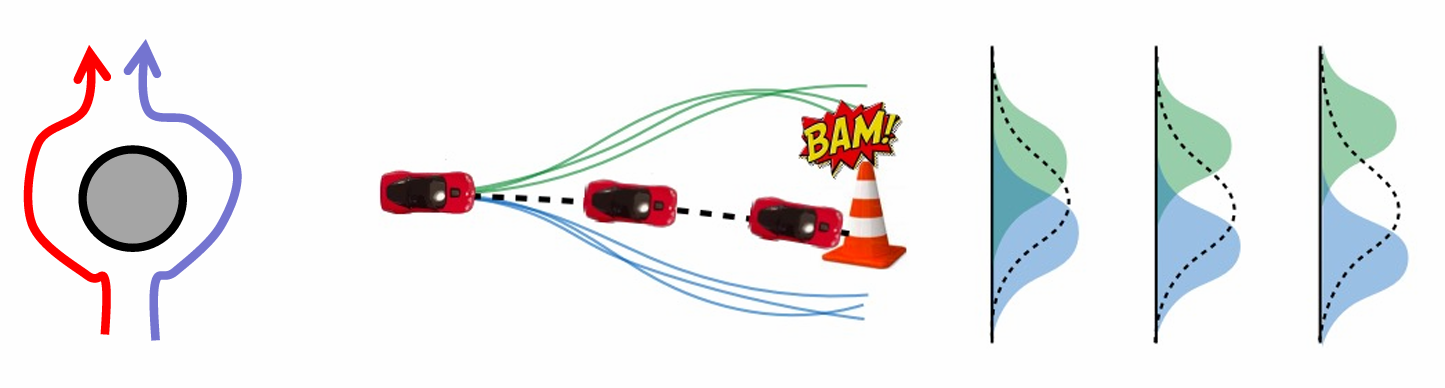
\includegraphics[width=0.9\linewidth]{rl/modeavg.png}
        \caption{An illustration demonstrating the issues that arise from mode-averaging within behavior cloning algorithms. The green and blue peaks represent choosing to go left or right around the obstacle, and the black dashed line represents what a simple policy will converge on.}
        \label{fig:modeavg}
    \end{figure}
\end{flushleft}

\section{Proofs for Problems with Behavior Cloning}
% \subsection{Quadratically Compounding Error}
% \begin{flushleft}
%     \large Below is a walkthrough demonstrating how basic behavior cloning has quadratically compounding error: \break

%     To analyze the effects of deviation from the expert, we create a cost function that gives us 1 when the agent deviates from the expert and 0 otherwise. This will let us quantify the number of deviations from the expert throughout an episode. $a^*$ represents the action the expert policy ($\pi_e$) would take at time $t$: $a^* = \pi_e(s_t)$.

%     $$c(s_t, a_t) = \begin{cases} 
%           0, & \textrm{if } a_t = a^* \\
%           1, & \textrm{otherwise} 
%        \end{cases}
%     $$

%     We also assume the ``worst case scenario'', meaning that once the agent takes a decision that takes it off of the path of the expert, we have no guarantees that it will ever find its way back on track and penalize it heavily. The earlier it goes off track, the higher the penalty. A mistake at time $t = 0$ will incur a penalty of 1 for each subsequent timestep until the episode ends. We say that an episode has length $H$. So:

%     \begin{itemize}
%         \item If $a_t \neq a^*$  when $t=0$ $\rightarrow$ Cost = $H$
%         \item If $a_t \neq a^*$  when $t=1$ $\rightarrow$ Cost = $H-1$
%         \item If $a_t \neq a^*$  when $t=2$ $\rightarrow$ Cost = $H-2$
%         \item ...
%         \item If $a_t \neq a^*$  when $t=H-1$ $\rightarrow$ Cost = $1$
%         \item If $a_t \neq a^*$  when $t=H$ $\rightarrow$ Cost = $0$
%     \end{itemize}

%     We can write this in summation form as:

%     $$\sum_{t=0}^H \biggl[ \sum^{H-t} c(s_t, a_t)\biggr]$$

%     Because we know that $\pi_\theta$ is somewhat imperfect, we assign a probability $\epsilon$ which represents the chance that the agent picks an action different from the expert:

%     $$p(\pi_\theta(s_t) \neq a^*) = \epsilon$$

%     We finally take the expected value of the cost throughout an episode and bound it. We assume that $s_t$ and $a_t$ come from $\pi_\theta$:

%     $$\mathrm{Expected\;Cost} = \mathbb{E}\sum_{t=0}^H \biggl[ \sum^{H-t} c(s_t, a_t)\biggr]$$

%     We can use Linearity of Expectation (LOE) to move the expectation inside the summations:

%     $$\mathrm{Expected\;Cost} = \sum_{t=0}^H \biggl[ \sum^{H-t} \mathbb{E}[c(s_t, a_t)]\biggr]$$

%     The expected value of an indicator variable (in this case $c(s_t,a_t)$) is equal to the probability of that event ocurring. We said earlier that the probability the agent chooses an action different from the expert is $\epsilon$:

%     $$\mathrm{Expected\;Cost} = \sum_{t=0}^H \sum^{H-t} \epsilon$$

%     We can now create a quadratic upper bound:

%     \begin{align*}
%         \mathrm{Expected\;Cost} &= \sum_{t=0}^H \sum^{H-t} \epsilon \\
%         &= H\epsilon + (H-1)\epsilon + (H-2)\epsilon +...+ \epsilon + 0\\
%         &\leq H\epsilon + H\epsilon + H\epsilon +...+ H\epsilon\\
%         \mathrm{Expected\;Cost} &\leq H^2\epsilon
%     \end{align*}

%     Now we can clearly see that the expected error over an episode with length $H$ can be quadratically compounding.
% \end{flushleft}

\subsection{Mode Averaging}
\begin{flushleft}
    \large Below is a walkthrough demonstrating how mode-averaging comes out as a problem in behavior cloning: \break

    Take our original behavior cloning objective

    $$\underset{\theta}{\textrm{argmax}}\biggl[\mathbb{E}_{(s^*,a^*) \sim \mathcal{D}}[\mathrm{log}\pi_\theta(a^*|s^*)]\biggr]$$

    We define $\pi_e$ as the expert policy. Under the expectation $\mathbb{E}_{(s^*,a^*) \sim \mathcal{D}}$, $\mathrm{log}\pi_e(a^*|s^*) = 0$ is always true. This is because the expert policy will always assign $a^*$ (optimal action) a probability of 1 given a state $s^*$. $\pi_e(a^*|s^*) = 1$, $\mathrm{log}(1) = 0$, so  $\mathrm{log}\pi_e(a^*|s^*) = 0$. We can therefore insert into the equation:

    $$\underset{\theta}{\textrm{argmax}}\biggl[\mathbb{E}_{(s^*,a^*) \sim \mathcal{D}}[\mathrm{log}\pi_\theta(a^*|s^*) - \mathrm{log}\pi_e(a^*|s^*)]\biggr]$$

    Split the expectation into two nested expectations. $(s^*,a^*) \sim \mathcal{D}$ can be rewritten as $s^* \sim p_{\pi_e}(\cdot)$ followed by $a^* \sim \pi_e(\cdot|s^*)$. In english, this means we get a state $s^*$ by sampling from possible states the expert ($\pi_e$) has explored and then sample the action $a^*$ from the policy $\pi_e$ given that it considers $s^*$. The end result is the same, as we have the variables $s^*$ and $a^*$ to use, and they come from the expert.

    $$\underset{\theta}{\textrm{argmax}}\biggl[\mathbb{E}_{s^* \sim p_{\pi_e}(\cdot)}[\mathbb{E}_{a^* \sim \pi_e(\cdot|s^*)}[\mathrm{log}\pi_\theta(a^*|s^*) - \mathrm{log}\pi_e(a^*|s^*)]]\biggr]$$

    Invert the whole expression from an argmax to an argmin by multiplying by -1, which carries through all the expectations because $a\mathbb{E}[X] = \mathbb{E}[aX]$.

    $$\underset{\theta}{\textrm{argmin}}\biggl[\mathbb{E}_{s^* \sim p_{\pi_e}(\cdot)}[\mathbb{E}_{a^* \sim \pi_e(\cdot|s^*)}[\mathrm{log}\pi_e(a^*|s^*) - \mathrm{log}\pi_\theta(a^*|s^*)]]\biggr]$$

    Use properties of logarithms to rewrite the innermost term:

    $$\underset{\theta}{\textrm{argmin}}\biggl[\mathbb{E}_{s^* \sim p_{\pi_e}(\cdot)}[\mathbb{E}_{a^* \sim \pi_e(\cdot|s^*)}[\mathrm{log}\frac{\pi_e(a^*|s^*)}{\pi_\theta(a^*|s^*)}]]\biggr]$$

    For the final step, we must introduce the concept of F-divergence. An F-divergence is, in simple terms, a function that measures the ``distance'' between two functions. The general form of an F-divergence $D_f$ is:

    $$D_f(p(x),q(x)) = \mathbb{E}_{q(x)} \biggl[ f\biggl( \frac{p(x)}{q(x)}\biggr)\biggr]$$
    
    You may be familiar with Kullback-Leibler Divergence (KL divergence) which is a form of F-divergence. KL divergence quantifies the difference between two probability distributions. If you define an F-divergence with $f(x) = x\mathrm{log}(x)$, you get what is called the \textbf{forward KL divergence}.
    
    $$\mathrm{Forward\;KL\;Divergence} = D_{KL}(p(x),q(x)) = \mathbb{E}_{p(x)} \biggl[\mathrm{log}\frac{p(x)}{q(x)}\biggr]$$
    
    A quick proof of this fact is shown below. We use the property that $\mathbb{E}_{q(x)}[p(x)] = \int p(x)q(x)\;dx$.

    \begin{align*}
        \textrm{Given: }f(x) \leftarrow x\mathrm{log}x \\
        D_f(p(x),q(x))\ &= \mathbb{E}_{q(x)} \biggl[ \frac{p(x)}{q(x)}\mathrm{log}\frac{p(x)}{q(x)}\biggr]\\
        &= \int \frac{p(x)}{q(x)}\mathrm{log}\frac{p(x)}{q(x)}q(x)\;dx\\
        &= \int p(x)\mathrm{log}\frac{p(x)}{q(x)}\;dx\\
        D_{KL}(p(x),q(x)) &= \mathbb{E}_{p(x)} \biggl[\mathrm{log}\frac{p(x)}{q(x)}\biggr]
    \end{align*}

    We can apply the definition of forward KL divergence to the inner expectation shown before.

    $$\mathbb{E}_{a^* \sim \pi_e(\cdot|s^*)}[\mathrm{log}\frac{\pi_e(a^*|s^*)}{\pi_\theta(a^*|s^*)}] = D_{KL}(\pi_e(\cdot|s^*),\pi_\theta(\cdot|s^*))$$

    We are in this expression calculating the KL divergence between the expert policy action distribution given state $s^*$ and the agent's action distribution given state $s^*$. We can now insert this back into the original equation and draw some insights:

    $$\underset{\theta}{\textrm{argmax}}\biggl[\mathbb{E}_{(s^*,a^*) \sim \mathcal{D}}[\mathrm{log}\pi_\theta(a^*|s^*)]\biggr] = \underset{\theta}{\textrm{argmin}}\biggl[\mathbb{E}_{s^* \sim p_{\pi_e}(\cdot)}[D_{KL}(\pi_e(\cdot|s^*),\pi_\theta(\cdot|s^*))]\biggr]$$

    We now see the original behavior cloning problem formulation written as an F-divergence (more specifically, KL divergence) minimization problem. \textit{Since the F divergence is forward KL divergence, it is mode-averaging by nature}. In other words, trying to minimize the forward KL divergence between a multimodal expert policy $\pi_e$ and a single-mode actor policy $\pi_\theta$ will result in finding a policy that does not fit to either mode, but seeks to the mean of both. Seeing the KL divergence clearly in the equation makes this an unavoidable fact. This gives us a much more concrete basis for why we should expect to observe the crashing behavior discussed earlier!

    \begin{figure}[H]
        \centering
        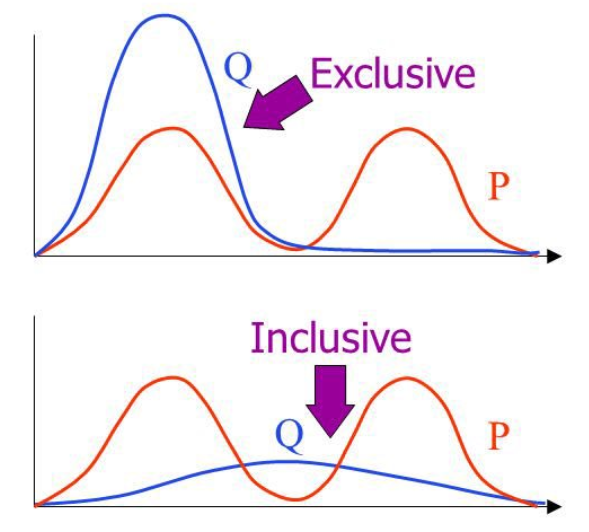
\includegraphics[width=0.7\linewidth]{rl/diffkl.png}
        \caption{The blue curve is our single-mode Gaussian decision policy and the bimodal orange line is our expert policy (can go left or right around the tree). The top graph shows what we would like to happen, which is choosing a mode and sticking with it. However, the bottom graph shows what actually happens when we minimize forward KL divergence. This is mode-averaging behavior (crashing into the tree).}
        \label{fig:diffkl}
    \end{figure}

    This analysis also gives us another avenue by which to improve behavior cloning instead of selecting a more expressive policy class: Find ways to rewrite the original objective such that we end up with a different F-divergence that is not mode-averaging. There are papers written about this that I suggest you read if you are very interested in this subsection of RL.
\end{flushleft}

\section{DAgger Algorithm}
\begin{flushleft}
    \large DAgger seeks to preserve the core of behavior cloning \textemdash\; learning by following an expert \textemdash\; but making it so that we are not on a ``precarious ledge'' and small perturbations do not send us way off track. DAgger stands for \textbf{\textit{D}ataset \textit{A}ggregation}, and improves the performance of behavior cloning by augmenting $\mathcal{D}$ with more human data, but intelligently. \break

    A basic DAgger algorithm will look like the following:
    \begin{enumerate}
        \item Train $\pi_\theta$ (initial policy) on examples from $\mathcal{D}$, the dataset of examples from the expert
        \item Run the policy $\pi_\theta$ and record the trajectory $\tau = (s_0, a_0, s_1, a_1...)$ or the actions it takes in a sequence
        \item Have a human label each $s_t \in \tau$ with the optimal action $a^*$. Call all these $(s, a)$ pairs $\mathcal{D}_{\pi_\theta}$
        \item Add $\mathcal{D}_{\pi_\theta}$, or the new state action pairs, to $\mathcal{D}$. $\mathcal{D} \leftarrow \mathcal{D} \cup \mathcal{D}_{\pi_\theta}$. The datasets have been aggregated!
        \item Repeat until the agent behaves well.
    \end{enumerate}

    Why does this work well? In essence, you are ``extending the precarious ledge'' that behavior cloning usually creates. A human adding corrective labels at critical failure points lets the agent know what to do at those points to get back on track.

    \begin{figure}[H]
        \centering
        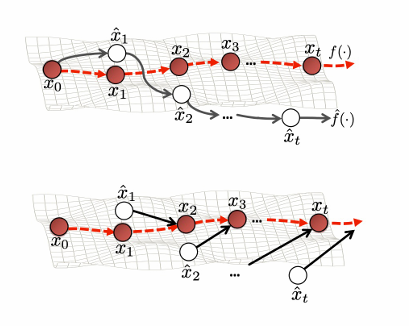
\includegraphics[width=0.7\linewidth]{rl/daggerviz.png}
        \caption{A visualization of how DAgger helps keep the agent performing well. We first see the agent ($\hat{x}$) deviate from the expert ($x$), but we then take these observations of where the agent failed and give it instructions on how to get back on track. With enough iterations, a lot of failure cases can be mitigated.}
        \label{fig:daggerviz}
    \end{figure}

    Behavior cloning is a section of RL that may seem simple at first, but can be quite involved when you try to solve the problems that come with a naive implementation. The next few sections will cover more ``core'' RL algorithms and analyze their strengths/weaknesses.
\end{flushleft}

\begin{questionbox}
\textbf{Synthesis Questions:}
\begin{enumerate}
    \item Write definitions for the following symbols:
    \begin{itemize}
        \item $(s_t, a_t)$
        \item $(s^*, a^*)$
        \item $\mathcal{D}$
    \end{itemize}
    \item What does the $\theta$ in $\pi_\theta$ represent?
    \item What is the issue of \textit{quadratically compounding error} in behavior cloning, and how does DAgger mitigate it?
    \item What is the issue of \textit{mode averaging} in behavior cloning, and how do you prevent it from happening?
\end{enumerate}
\end{questionbox}


\section{Policy Gradient}
\subsection{Basic Policy Gradient}
\begin{flushleft}

    \begin{figure}[H]
            \centering
            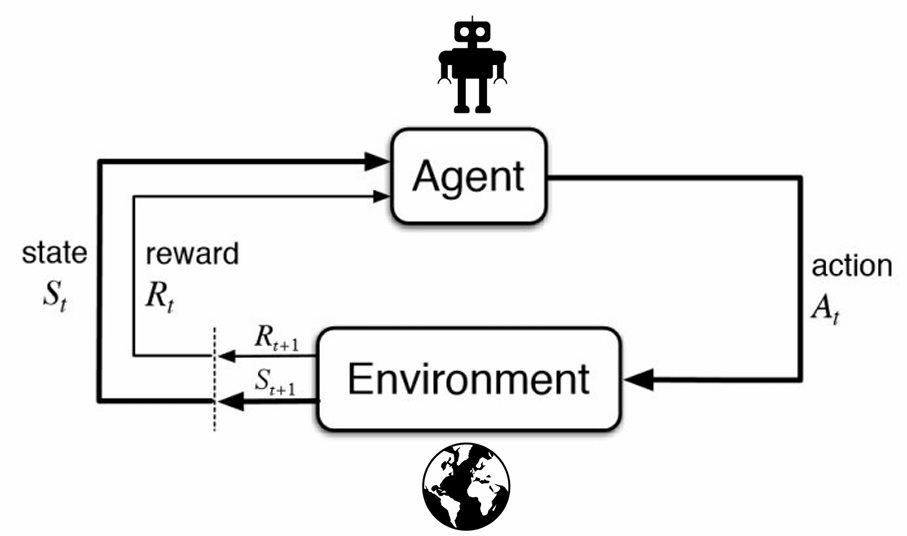
\includegraphics[width=0.7\linewidth]{rl/rlsystem.png}
            \caption{An illustration showing how the agent and environment communicate through actions, states, and rewards in a traditional RL setting. The subscript $t$ is for timestep.}
            \label{fig:rlsystem}
    \end{figure}
    
    \large Let's start by introducing a new problem scenario. in this hypothetical, we do \textit{not} have an expert to learn from. Instead, we receive \textbf{rewards} from the environment. This is the more traditional RL problem setup we discussed earlier. In this case, we have to define a new objective function that is based on rewards, not expert state-action pairs. Lets just do the simplest thing and try to \textit{maximize the rewards} that the agent receives over time. How can we write this down? Well, the sum of rewards an agent receives over the course of a trajectory is called the \textbf{return} of that trajectory. It is denoted as $R(\tau)$. It can have a few different formulations. Here is the one that will be important for policy gradient (PG): \break

    \textbf{Infinite Horizon Discounted Reward:}
    $$R(\tau) = \sum_{t=0}^\infty \gamma^t r(s_t, a_t)$$

    The $s_t$ and $a_t$ come from the trajectory $\tau$. We simply add up all the rewards throughout the trajectory, but reducing the contribution of $r(s_t,a_t)$ way in the future through the use of the discounting factor $\gamma$ (usually around 0.85-0.99). This is because we don't value the future returns as much as immediate ones. As $t \rightarrow \infty$, $\gamma^t \rightarrow 0$. This ensures that really long trajectories don't result in a incalculably large return. For example, a reward of 100 at $t = 0$ contributes 100 to the sum, but if the same reward is received 25 steps in the future, or at timestep $t = 25$ with $\gamma = 0.95$, a reward of 100 only contributes about $0.95^{25}\cdot100 \approx 27$ to the sum. By timestep $t = 1000$, rewards are not even considered. \break

    We can now be more specific about our objective. We want to \textit{maximize the return that the agent receives}. Here is how we do it. We first create an equation that has policy parameters as its input. We want this function to give us the expected return if we were to use a policy with these parameters. Now we want to find the perfect parameters $\theta$ that gives us the highest return. We can do this by performing \textbf{gradient ascent} on the parameters. This is why the method is called policy gradient! \break

    Below is the equation we want to maximize using gradient ascent:

    $$J(\theta) = \mathbb{E}_{\tau \sim \pi_\theta} [R(\tau)]$$

    In English: Maximize the expected ($\mathbb{E}$) return of trajectories ($R(\tau)$) explored ($\tau \sim \pi_\theta$) by the agent by adjusting the parameters of the model ($\theta$). The model in this case would be a neural network so $\theta$ represents weights and biases. \break
    
    Our ultimate goal is to calculate $\nabla_\theta J(\theta)$ and \textbf{update} $\theta$ as such on each iteration $i$:

    $$\theta_{i+1} \leftarrow \theta_i + \nabla_\theta J(\theta)$$

    If we repeat this process many times, we should have parameters to a policy that gives you high returns. This means that our agent will be ``playing'' the game properly, and Mario will reach the flagpole! \break

    The proof for this is later in the article, but calculating the gradient of $J(\theta)$ gives us the following:

    $$\nabla_\theta J(\theta) \approx \frac{1}{N}\sum_{i=0}^N\sum_{t=0}^T\biggl[ \nabla_\theta \mathrm{log}\pi_\theta(a_t^i|s_t^i)\sum_{t'=0}^T \gamma^{t'} r(s_{t'}^i, a_{t'}^i)\biggr]$$

    It seems complicated, but it means something quite intuitive. Firstly, the $\approx$ exists because this is a ``Monte-Carlo'' approximation to the \textit{actual} gradient, which is in an expectation. Evaluating this would mean exploring every single possible trajectory, which is impossible for anything but toy problems. This is what the outer sum $\frac{1}{N}\sum_{i=0}^N$ signifies: Try a few trajectories and average your results, as opposed to checking all of them. It is similar in principle to stochastic gradient descent (SGD). \break

    The inner summation is where the meat of PG lies. Notice that there are two $t$ variables, $t$ and $t'$. The summation regarding $t'$ is just the expanded form of the return we saw earlier. This is a ``weight'' or ``scaler'' for the very important term $\nabla_\theta \mathrm{log}\pi_\theta(a_t^i|s_t^i)$. This term represents the gradients of the log-likelihood of taking action $a_t$ given $s_t$ under policy $\pi_\theta$. That is a bit confusing, but here is the important bit: \textit{The higher this value is, the more likely the policy will be to take this same trajectory again after performing an update}. This is why we weight it by the return. \break
    
    (1) A high return, say 100, indicates that the agent was on a good trajectory. We want to increase the chances we take these same actions at these same states by a lot. So we scale the gradients by 100 (the return). After an update to the weights, our policy $\pi_\theta$ is much more likely to find that good trajectory again. (2) Now say the agent blunders and gets a trajectory with a return of 5. This is not very good, so we don't really want to take these same actions in the same states again. Not much about the model changes. (3) Now say the agent does very poorly and gets a return of -99. This is terrible! We actually push the gradients in the opposite direction, making $\pi_\theta$ less likely to make the same blunders that got us such a low return after a parameter update. \break

    Actually calculating this derivative $\nabla_\theta \mathrm{log}\pi_\theta(a_t^i|s_t^i)$ is taken care of by autodiff within PyTorch, TensorFlow, or the deep learning library of your choice. You don't need to worry about the computation too much. Doing a forward pass through the network lets the library create a computation graph (what operations happened and in what order) to then calculate gradients for the parameters $\theta$. In short: the actual derivative is done for you. The trick of PG is scaling it by the return to make actions in good trajectories more likely to occur. Do this over and over again $N$ times and perform an update. Perform many updates and you will get an agent that can play a complex game!
\end{flushleft}
\section{Advanced Policy Gradient Concepts}
\subsection{Return-to-Go}
\begin{flushleft}
    \large Despite seeming complex enough, Vanilla PG suffers from a few problems: The biggest of them being that Vanilla PG is a \textbf{high-variance estimator}. What this means is that you could train the model 100's of times and change nothing but the random seed used to initialize the weights, but get 99 failures and one success. It will not train nor work consistently most of the time. Therefore more advanced PG methods attempt to reduce the variance of the estimator. \break

    The simplest of these advances is something called \textbf{return-to-go} estimation. It deals with this part of the PG gradient:

    $$\sum_{t'=0}^T \gamma^{t'} r(s_{t'}^i, a_{t'}^i)$$

    Notice that $t'$ will sum from 0 to $T$, regardless of what value $t$ is at in the middle summation. What this means is that, even when we are calculating gradients for $\mathrm{log}\pi_\theta(a_10|s_10)$, we are scaling them by rewards gained from timesteps 0 to 9. This is nonsensical, because actions at time $t=10$ cannot affect the past! As such, we make a slight adjustment to the formula for the PG gradient:

    $$\nabla_\theta J(\theta) \approx \frac{1}{N}\sum_{i=0}^N\sum_{t=0}^T\biggl[ \nabla_\theta \mathrm{log}\pi_\theta(a_t^i|s_t^i)\sum_{t'=t}^T \gamma^{t'} r(s_{t'}^i, a_{t'}^i)\biggr]$$

    Notice that in the third summation, we changed from $t'=0$ to $t'=t$.
\end{flushleft}
\subsection{Baseline Function}
\begin{flushleft}
    \large Another way to reduce the variance of the estimator (without increasing the bias) is to subtract a \textbf{baseline function} ($b(s_t)$) from the return. Due to how PG collects samples to train on, scale variation between returns of trajectories makes the policy gradient unstable. Assume that the average reward through all trajectories is 10. A ``good'' trajectory would have a return 15, and a bad trajectory would have a return of 5. However, due to the fact that these are both positive, the probabilities of taking actions that lead to these trajectories would \textit{both} be increased, as opposed to increasing one and decreasing the other. A baseline fixes this by centering returns around 0.

    $$\nabla_\theta J(\theta) \approx \frac{1}{N}\sum_{i=0}^N\sum_{t=0}^T\biggl[ \nabla_\theta \mathrm{log}\pi_\theta(a_t^i|s_t^i)\biggl(\biggl(\sum_{t'=t}^T \gamma^{t'} r(s_{t'}^i, a_{t'}^i)\biggl) - b(s_t)\biggr)\biggr]$$

    The simplest baseline function is represented by $\bar{R}$, which just is the average reward over the sampled trajectories:

    $$\bar{R} = \frac{1}{N}\sum_{i=0}^N \sum_{t=0}^T r(s_t^i,a_t^i)$$

    More complex baseline functions can be more effective, but begin to blend the line between PG and another RL algorithm (Actor-Critic). \break
\end{flushleft}
\subsection{Natural Policy Gradient}
    \begin{flushleft}
    \large The final PG improvement we will be covering (in brief) is Natural Policy Gradient (NPG). A large issue that comes up within PG methods is overshooting the true gradient. Remember the $\approx$ sign we introduced? That was because we sample $N$ trajectories and compute an \textit{approximate} gradient to take a step. Agent performance is very sensitive to small changes in the policy, so misstepping in a parameter update could make the model completely collapse. We could choose a very small step size, but this makes model training take much longer. Instead, we add an additional constraint to our optimization. The notation for this is a bit confusing, but the general idea is to add the following constraint:

    $$D_{KL}(\pi_\theta|\pi_{\theta_i}) \leq \epsilon$$

    What we are saying here is that we want the difference between how the policy behaves \textit{before} vs. \textit{after} a gradient step to be \textit{constrained} by $\epsilon$. This helps us reduce the chance that a huge misstep occurs and throws our agent off track. We constrain our gradient to push us in a better direction without sacrificing step size! The implementation of this is beyond the scope of the article so we will not be covering it. \break

    \begin{figure}[H]
        \centering
        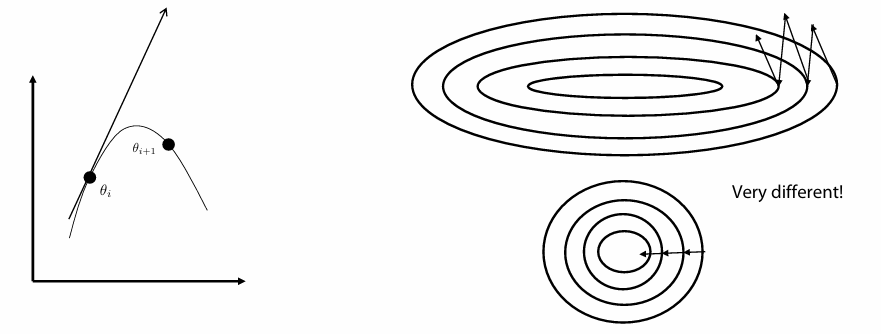
\includegraphics[width=0.9\linewidth]{rl/npg.png}
        \caption{There are a few items in this diagram. The parabola and tangent show the issues of large gradient steps when you have only a monte-carlo approximation to the true gradient. You can wildly overshoot where you should be ($\theta_{i+1}$).The dimensions of the stretched oval represent the parameters of the policy, and how steps in the wrong direction can be disastrous since the policy is very sensitive to small parameter shifts. What we don't have in RL is an easy objective to optimize on like the circle. These problems together are why NPG is useful.}
        \label{fig:npg}
    \end{figure}

    Very advanced PG methods build off of NPG, and include trust region policy optimization (TRPO) and proximal policy optimization (PPO). PPO was the RL algorithm used to finetune ChatGPT, and is generally very powerful. I suggest looking into both of these methods if you are interested in exploring policy gradient methods more.
\end{flushleft}

\subsection{Proof for Gradient of the PG Objective}
\begin{flushleft}
    \large Below is a walkthrough demonstrating how to calculate the gradient of the policy gradient objective function: \break

    We first take a look at the function we want to calculate the gradient with respect to $\theta$ for:

    $$J(\theta) = \mathbb{E}_{\tau \sim \pi_\theta}[R(\tau)]$$

    In English: $J(\theta)$ is the expected return of trajectories ($R(\tau)$) explored ($\tau \sim \pi_\theta$) by the agent. Remember that $\theta$ represents the weights and biases of a neural network. \break
    
    We cannot easily compute the gradient in this expectation form since $\pi_\theta$ is nowhere to be seen in the equation. Through some clever algebra tricks we can change how the expression looks and take the gradient. Let's write the expectation in integral form: \break

    $$J(\theta) = \int R(\tau)p_{\theta}(\tau)\;d\tau$$

    The term $p_\theta(\tau)$ is the probability of encountering trajectory $\tau$ while the policy has parameters $\theta$. Now let's introduce the gradient and move it inside the integral:

    \begin{align*}
        \nabla_\theta J(\theta) &= \nabla_\theta\int R(\tau)p_{\theta}(\tau)\;d\tau \\
        \nabla_\theta J(\theta) &= \int \nabla_\theta R(\tau)p_{\theta}(\tau)\;d\tau
    \end{align*}
    
    Now what do we do? Here is where something called the ``REINFORCE'' trick comes into play I will break it down very clearly below and then explain how it works:

    \begin{align*}
        \nabla_\theta J(\theta) &= \int \nabla_\theta R(\tau)p_{\theta}(\tau)\;d\tau \\
        &= \int \nabla_\theta p_{\theta}(\tau)R(\tau)\;d\tau \\
        &= \int \frac{p_{\theta}(\tau)}{p_{\theta}(\tau)}\nabla_\theta p_{\theta}(\tau) R(\tau)\;d\tau \\
        &= \int p_{\theta}(\tau)\frac{1}{p_{\theta}(\tau)}\nabla_\theta p_{\theta}(\tau) R(\tau)\;d\tau \\
        &= \int p_{\theta}(\tau) \nabla_\theta \mathrm{log}(p_\theta(\tau)) R(\tau)\;d\tau \\
        \nabla_\theta J(\theta) &= \mathbb{E}_{\tau \sim p_\theta(\tau)}[\nabla_\theta \mathrm{log}(p_\theta(\tau)) R(\tau)] 
    \end{align*}

    We first multiply by $\frac{p_{\theta}(\tau)}{p_{\theta}(\tau)}$, which is equivalent to one and does not imbalance the equation. We then use the fact that $\nabla \mathrm{log}(f(x)) = \frac{1}{f(x)}\nabla f(x)$ from the chain rule and replace some terms. We finally use the definition of expectation to transform the integral back to an expectation with respect to $\tau \sim p_\theta(\tau)$. \break

    Now we focus on the $\nabla_\theta \mathrm{log}(p_\theta(\tau))$, expanding, cancelling, then contracting to arrive at our final result. It is important to understand what exactly $p_\theta(\tau)$ exactly is. In English, it is the probability of encountering trajectory $\tau$ while operating under policy $\pi_\theta$. It can be written out in long form as such:

    $$p_\theta(\tau) = p(s_0) \prod_{t=0}^{T-1} \pi_\theta(a_t|s_t)p(s_{t+1}|s_t,a_t)$$

    We take the probability of being in state $s_0$ from the trajectory to start the product chain. We multiply it by $\pi_\theta(a_0|s_0)$, the probability that the agent took action $a_0$ from the trajectory given being in state $s_0$. We also consider the probability of transitioning from state $s_0 \rightarrow s_1$ given that action $a_0$ was taken. This is decided by the environment, not the agent. We then keep multiplying these terms together from $t=0$ to $T-1$. We now introduce the logarithm, which transforms the equation a bit:

    $$\mathrm{log}(p_\theta(\tau)) = \mathrm{log}(p(s_0)) + \sum_{t=0}^{T-1} \mathrm{log}(\pi_\theta(a_t|s_t)) + \mathrm{log}(p(s_{t+1}|s_t,a_t))$$

    The properties of logarithms ($\mathrm{log}(ab) = \mathrm{log}(a) + \mathrm{log}(b)$) transform this product into an easy-to-derive sum. We now apply the gradient:
    
    \begin{align*}
        \nabla_\theta \mathrm{log}(p_\theta(\tau)) &= \nabla_\theta \biggl(\mathrm{log}(p(s_0)) + \sum_{t=0}^{T-1} \mathrm{log}(\pi_\theta(a_t|s_t)) + \mathrm{log}(p(s_{t+1}|s_t,a_t))\biggr)\\
        &= \nabla_\theta \mathrm{log}(p(s_0)) + \sum_{t=0}^{T-1} \nabla_\theta\mathrm{log}(\pi_\theta(a_t|s_t)) + \nabla_\theta\mathrm{log}(p(s_{t+1}|s_t,a_t)) \\
        &= \sum_{t=0}^{T-1} \nabla_\theta\mathrm{log}(\pi_\theta(a_t|s_t))
    \end{align*}

    When we take the gradient with respect to $\theta$ ($\nabla_\theta$), we can eliminate any terms that do not concern $\theta$. This is how we were able to get rid of $p(s_0)$ and $\mathrm{log}(p(s_{t+1}|s_t,a_t))$. Getting rid of this second term is especially crucial, because it makes our method \textbf{model-free}. We do not need to consider or try to model environment dynamics at all with this approach! Now we plug $\nabla_\theta \mathrm{log}(p_\theta(\tau))$ back into the larger equation, and expand $R(\tau)$:

    \begin{align*}
        \nabla_\theta J(\theta) &= \mathbb{E}_{\tau \sim p_\theta(\tau)}[\nabla_\theta \mathrm{log}(p_\theta(\tau)) R(\tau)] \\
        &= \mathbb{E}_{\tau \sim p_\theta(\tau)}\biggl[\sum_{t=0}^{T-1} \nabla_\theta\mathrm{log}(\pi_\theta(a_t|s_t))R(\tau)\biggr]\\
        &= \mathbb{E}_{\tau \sim p_\theta(\tau)}\biggl[\sum_{t=0}^{T-1} \nabla_\theta\mathrm{log}(\pi_\theta(a_t|s_t))\sum_{t'=0}^T \gamma^{t'} r(s_{t'}, a_{t'})\biggr]
    \end{align*}

    And now, we create a Monte-Carlo approximation to the expectation by sampling trajectories, and we arrive at the PG gradient we introduced earlier! Note the change from $T-1$ to $T$, we do this for ease of understanding and since we are already approximating the true gradient the impact is minimal.

    $$\nabla_\theta J(\theta) \approx \frac{1}{N}\sum_{i=0}^N\sum_{t=0}^T\biggl[ \nabla_\theta \mathrm{log}\pi_\theta(a_t^i|s_t^i)\sum_{t'=0}^T \gamma^{t'} r(s_{t'}^i, a_{t'}^i)\biggr]$$
\end{flushleft}

\begin{questionbox}
\textbf{Synthesis Questions:}
\begin{enumerate}
    \item What is infinite-horizon discounted reward, and why is it important?
    \item Answer the following questions about $\gamma$, a term within the formulation for infinite-horizon discounted return.
    \begin{itemize}
        \item What is $\gamma$?
        \item What would a low value of $\gamma$ do to rewards in the far future?
        \item Give one scenario where a low $\gamma$ is good, and one where a high $\gamma$ is good.
        \item Why cant $\gamma$ be $\geq$ 1?
    \end{itemize}
    \item What is $J(\theta)$, and what do we want to do with it?
    \item How does policy gradient improve the performance of the policy? In other words, how do we get the probabilities of good actions given a specific state to go up?
    \item Explain how the following ``tricks'' reduce the variance of policy gradient and make it more stable.
    \begin{itemize}
        \item Return-to-Go
        \item Baseline functions
        \item Natural policy gradient/constrained optimization
    \end{itemize}
\end{enumerate}
\end{questionbox}


\section{Deep Q-Learning}
\subsection{Q-Functions and Bellman Equations}
\begin{flushleft}
    \large Q-Learning will introduce us to our first off-policy RL algorithm, and is the first step into a whole other realm of RL algorithms. Many of these algorithms use language or ideas captured within Q-Learning, which is why we discuss it. \break

    The main idea behind Q-Learning is that we want to create a ``Quality Function'' that can evaluate state-action pairs. Given some state and an action in that state, we should get a number that tells us how good things will play out in the future if we were to take this action. In other words, what is the expected return from time $t$ and onward, if we take action $a_t$ in state $s_t$, and then follow policy $\pi_\theta$ from then on out? This function is usually approximated by a neural network. We will note this by parameterizing the Q-function with $\phi$ to represent the weights and biases of the network. We can write this all out as such below:

    $$Q_\phi^\pi(s, a) = \mathbb{E}_{\tau \sim \pi_\theta} \biggl[\sum_{t' = t}^T \gamma^{t'}r(s_{t'}, a_{t'}) | s_t = s,\;a_t = a\biggr]$$
    
    Note that the state-action pair $(s_t, a_t)$ is given to the equation, but all other state-action pairs come about as a consequence of following policy $\pi_\theta$ afterwards. \break

    \begin{figure}[H]
        \centering
        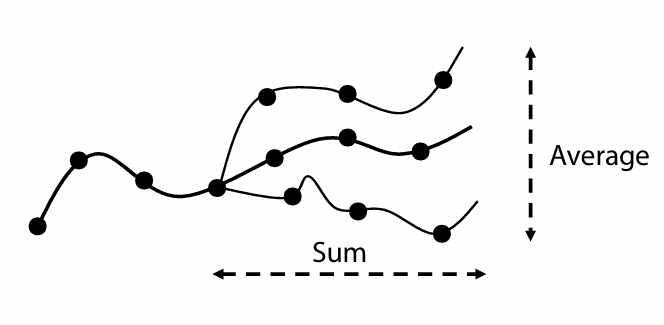
\includegraphics[width=0.7\linewidth]{rl/qlearning.png}
        \caption{A visualization of what the Q-function takes into account. It averages the rewards from time $t$ and forward across considers many paths that policy $\pi_\theta$ could theoretically take. The output of a Q-function is called a Q-value. It signifies the ``quality'' of the given state-action pair.}
        \label{fig:qlearning}
    \end{figure}

    This might seem somewhat arbitrary, but it is an intuitive way to think about navigating an environment. Think about yourself. You evaluate what actions you have available to you by considering their impact on future events. You have the option to stay at home all day, and in the short term it would be rewarding. However, in the long term, you understand it is better to exercise and touch grass. your brain in a way has a well trained ``Quality Function'' embedded deep within it! \break
    
    Now we can expand this intuition and equation into an update rule. With some algebraic manipulation, we find that the Q-function actually has a \textbf{recursive property}.
    
    \begin{align*}
        Q_\phi^\pi(s_t, a_t) &= \mathbb{E}_{\tau \sim \pi_\theta} \biggl[\sum_{t' = t}^T \gamma^{t'}r(s_{t'}, a_{t'}) | s_t, a_t\biggr]\\
        & = r(s_t, a_t) + \mathbb{E}_{\tau \sim \pi_\theta} \biggl[\sum_{t' = t+1}^T \gamma^{t'}r(s_{t'}, a_{t'}) | s_{t+1} \sim p(\cdot|s_t,a_t),\;a_{t+1} \sim \pi_\theta(s_t) \biggr]\\
        & = r(s_t, a_t) + Q_\phi^\pi(s_{t+1}, a_{t+1})
    \end{align*}
    
    The ``$ s_{t+1} \sim p(\cdot|s_t,a_t),\;a_{t+1} \sim \pi_\theta(s_t)$'' part of the equation just shows where $s_{t+1}$ and $a_{t+1}$ come from: transition dynamics and the policy $\pi_\theta$ respectively. \break
    
    The recursive nature of the Q-function means it can be called a \textbf{Bellman equation}. This being true is a necessary condition for optimal behavior. If we got our hands on a ``perfect'' Q-function like this, where $Q_\phi^\pi(s_t, a_t)$ \textit{is really always equal to} $r(s_t, a_t) + Q_\phi^\pi(s_{t+1}, a_{t+1})$, then we call it $Q^*$ and can simply query it for the best action in any state. We would be able to act optimally always. However, this is not what we have our hands on. We have a neural network that needs to be trained to have similar behavior to the perfect $Q^*$. How can we accomplish this? It seems impossible due to the recursive nature of the equation. However, we can employ a trick here. \break
    
    We would like it to be true that $Q_\phi^\pi(s_t, a_t) = r(s_t, a_t) + Q_\phi^\pi(s_{t+1}, a_{t+1})$. This is an \textit{equation}, so both sides are equal and their difference \textit{should} be 0. So if we make our ``surrogate goal'' to be minimizing the difference between the two sides, then the Q-function we learn will obey this recursive property (to some degree) implicitly! We define this difference as ``surprise'', or TD-error, and denote it as $\delta$. We also square the difference to ensure it is always positive. \break
    
    $$\delta = \biggl(Q_\phi^\pi(s_t, a_t) - (r(s_t, a_t) + Q_\phi^\pi(s_{t+1}, a_{t+1}))\biggr)^2$$
    
    Again: minimizing $\delta$ will give us the ideal Q-function and allow the agent to navigate the environment while maximizing returns.
    
    \begin{align*}
        & \underset{\phi}{\mathrm{argmin}}\;\mathbb{E}_{\tau \sim \pi}[\delta]\\
        & \underset{\phi}{\mathrm{argmin}}\;\mathbb{E}_{\tau \sim \pi}\biggl[\biggl(Q_\phi^\pi(s_t, a_t) - (r(s_t, a_t) + Q_\phi^\pi(s_{t+1}, a_{t+1}))\biggr)^2\biggr]
    \end{align*}
    
    This is naturally off-policy, as the policy that $\tau$ comes from and the policy that $Q^\pi$ operates off of do \textit{not} need to be the same.
\end{flushleft}

\section{Making Q-Learning Work}
\subsection{Replay Buffer and Memory}
\begin{flushleft}
    \large One of the main benefits of an off-policy algorithm are that we can use data from old trajectories many times instead of once. Since the policy that $\tau$ comes from in the optimization objective does not need to be the same as the actor's policy, we can replace $\tau \sim \pi$ with $\tau \sim \mathcal{D}$, where $\mathcal{D}$ is just a database of stored trajectories. This is usually implemented as a \textbf{replay buffer}. Essentially, the last 100 to 1000 trajectories are stored in a circular queue, and you sample $N$ datapoints from this buffer to train on. You update the Q-function, and then run the agent in the environment to collect more trajectories for your queue. Very old trajectories are eventually thrown out as they probably amount to nothing better than a random search. However, as the model gets better, the data within $\mathcal{D}$ gets richer and more interesting. Perhaps the agent progresses farther in whatever level it is trying to beat and encounters new areas it didn't see before. This \textbf{``memory''} the agent has at it's disposal allows it to learn faster and have greater sample efficiency.

    $$\underset{\phi}{\mathrm{argmin}}\;\mathbb{E}_{\tau \sim \mathcal{D}}\biggl[\biggl(Q_\phi^\pi(s_t, a_t) - (r(s_t, a_t) + Q_\phi^\pi(s_{t+1}, a_{t+1}))\biggr)^2\biggr]$$
\end{flushleft}
\subsection{Optimization Stability and Polyak Averaging}
\begin{flushleft}
    \large By now you may still have a little skepticism on how we can improve $Q^\pi_\phi$ if it is being compared not to a ground truth, but mainly to itself. \textit{This is an issue that Q-Learning has, it is very unstable since the optimization objective changes constantly.} The Q-function learning from itself is like the ``blind leading the blind'' in a way. This is where we make small adjustments to the objective. We introduce $Q^\pi_{\hat{\phi}}$, which is a second Q-function we use to improve the stability of our optimization loop:

    $$\underset{\phi}{\mathrm{argmin}}\;\mathbb{E}_{\tau \sim \mathcal{D}}\biggl[\biggl(Q_\phi^\pi(s_t, a_t) - (r(s_t, a_t) + Q_{\hat{\phi}}^\pi(s_{t+1}, a_{t+1}))\biggr)^2\biggr]$$

    It takes the place of the ``target'' Q-function, the one that processes $(s_{t+1}, a_{t+1})$. Having a second Q-function here makes the optimization more stable, as we can control how fast it is updated using \textbf{polyak averaging}. Polyak averaging is a way to slow how fast the target Q-function changes its weights. A slower change means a more stable optimization loop.

    $$\hat{\phi} \leftarrow (1-\kappa)\phi + \kappa\hat{\phi}$$

    $\kappa$ controls the speed of the update, with higher numbers slowing the speed at which $\hat{\phi}$ approaches the same weights and biases as $\phi$.
\end{flushleft}
\subsection{Explore vs. Exploit and epsilon-Greedy Search}
\begin{flushleft}
    \large One of the final small concepts to discuss is not actually unique to Q-Learning or even RL, but benefits them greatly and is worth talking about. In RL, we can have \textbf{explore vs. exploit} problems crop up. We want to act optimally as much as possible, but we will never truly know if we are acting optimally unless we search through every possible route. However if we do this, then many of our actions would be wasted on sub-optimal routes that turn out to be duds that do not improve our return. We need to strike a balance. We should explore enough so that we are confident that we have found the best path, and then immediately switch to following that path. \break

    If you just always follow the policy as you train an agent, then the agent may never find the most optimal route. This is because the agent pigeonholes itself into something it perceives as optimal, but only because it does not know any better. For example, say that we ask an agent to solve a maze. The fastest way to actually get to the goal would be to go around the outside of the maze to reach it. However, our reward schema penalizes moving away from the goal and rewards going towards it. As such, the agent will never learn the behavior of backing up and taking temporary low reward for future high rewards and a speedy victory. It will always move forward into the maze since that is what gives the most reward upfront. \break

    We can combat this issue with an \textbf{$\epsilon$-greedy search strategy}. It is actually quite simple. With probability $\epsilon$, take a random action instead of the one the policy says to take. Start this probability quite high, and slowly reduce it to 0 over time. This makes the first part of the agent's training cycle random exploration. It is through this random exploration that the agent may stumble upon efficient solutions, such as going around the maze. \break
    
    Implementing $\epsilon$-greedy can allow an agent to randomly encounter paths it would not have encountered if it just followed what it thought was the ``best way forward''. Somewhat counterintuitively, one powerful way to improve performance in RL is to actually throw out all of the fancy mathematical formulation for a bit and just throw some dice on which paths to take. These paths can be much better in the long run for the agent. Perhaps there is a life lesson in here somewhere?
\end{flushleft}

\begin{questionbox}
\textbf{Synthesis Questions:}
\begin{enumerate}
    \item What does the Q-function accept, and what does it return? Why would having this be useful for an agent navigating an environment?
    \item A similar function to the Q-function exists, called the \textbf{Value function}. It is written as:
    $$V^\pi(s) = \mathbb{E}_{\pi_\theta} \biggl[ \sum_{t' = t}^T \gamma^{t'}r(s_{t'}, a_{t'}) | s_t = s\biggr]$$
    Do the following:
    \begin{itemize}
        \item Compare and contrast this function to the Q-function. What purpose do you think it could serve?
        \item Prove that this is a Bellman equation.
    \end{itemize}
    \item What is ``surprise'' or TD-error? Why does minimizing it allow us to learn a good Q-function?
    \item Why is Q-learning off-policy, and why is this a good thing?
    \item How does a replay buffer improve sample efficiency?
    \item Why do we use a target network and polyak averaging when training Q-learning algorithms?
    \item Write in your own words the explore vs. exploit problem, and explain how $\epsilon$-greedy search mitigates this issue.
\end{enumerate}
\end{questionbox}

\section{When to Use Reinforcement Learning}
\begin{flushleft}
    \large Deep reinforcement learning is relatively situational, and can be very unstable to train. It unfortunately takes a lot of compute, hyperparameter tuning, and general trial-and-error to get something to behave ``properly''. RL algorithms, like all AI applications, are error prone. In classification or regression tasks this is to be expected and can be mitigated, but if an RL algorithm is deployed in a robot then a failure can lead to disastrous consequences. \break
    
    Regardless, RL by design more closely mimics human behavior and can perhaps be used in the future along with guardrails to accomplish very complex tasks. It is also the method of choice when the problem you are trying to solve is ``game-like'' in nature. For example, playing a videogame. It is actually easier to use RL in this case than it would be to try and use other techniques. The primary avenue to explore RL further is research at the moment, but personal projects are also very possible (and impressive!). It is difficult but not impossible to incorporate RL into student projects with just the techniques in this article. A deeper understanding of RL requires a lot of math and reading, but you can do it!
\end{flushleft}

\section{Conclusion (RL)}
\begin{flushleft}
    \large This section covered basic RL concepts, introducing common notation and 4 major algorithms (Behavior Cloning, DAgger, Policy Gradient, Q-Learning). We also went over the drawbacks of some of these algorithms both intuitively and in depth. We also covered miscellaneous RL topics like markov decision processes (MDPs), on vs. off policy algorithms, and explore vs. exploit. RL models are capable of superhuman-like performance in game-style tasks if trained properly, which can be quite shocking to many. Understanding the basics of these algorithms can demystify their power and quell fears about their capabilities.
\end{flushleft}
